\begin{figure}
    \centering
    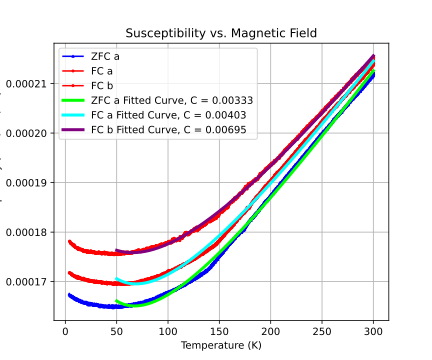
\includegraphics[width=\linewidth]{pdf_files/a_fitted_cw.pdf}
    \caption{ZFC a-axis, FC a-axis and FC b-axis data plotted together with fitted curves and extracted Curie Constant. The x-axis shows the temperature measured in Kelvin, the y-axis the volume susceptibility measured in emu/cm³/Oe.}
    \label{fig:a-fitted-cw}
\end{figure}